\chapter{Estudos de caso e anatomia da detecção}\label{estudo-de-caso-e-anatomia-da-detecuxe7uxe3o}
O exame longitudinal integra grandezas elétricas, cobertura, vínculo histórico e hipótese diagnóstica. O par de UCs da análise exploratória mostrou que a energia agregada pode ocultar diferenças importantes de forma e dispersão. Os casos a seguir ilustram o exame das evidências de mudança e das inconsistências de qualidade.
\section{Estudos de caso e hipóteses concorrentes}
Na UC 908***00, o cadastro registrou atualização em 31 de outubro, embora as medições anteriores permanecessem vinculadas ao mesmo NIO. Houve intervalo de indisponibilidade de dois dias e mudança persistente por 20 dias. A FA passou de 18,05 para 5,72 kWh/dia, queda aproximada de 68,3\%. Registrou-se RA em 12 dias posteriores, entre 14 e 31 kWh/dia nos dias com injeção. O escore elétrico individual atingiu 0,9601. A Figura \ref{caso} distingue os dois patamares de FA do intervalo de RA observado.

\begin{figure}[htbp]\centering\caption{Patamares de energia direta e faixa de energia reversa na UC 908***00}\label{caso}
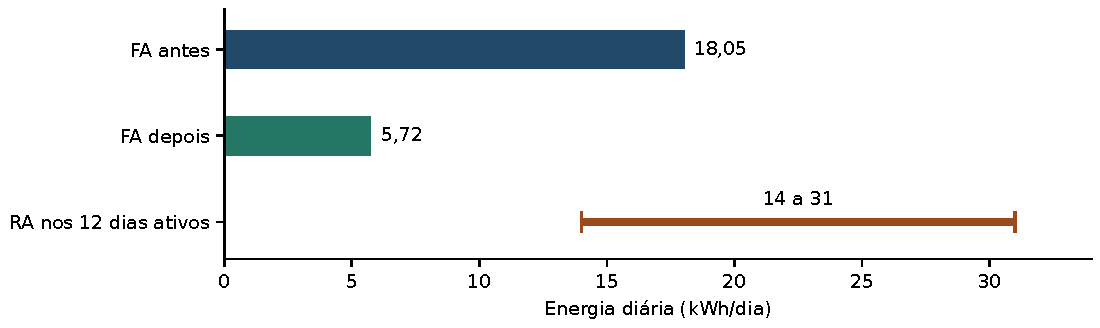
\includegraphics[width=0.96\textwidth,height=0.46\textheight,keepaspectratio]{figuras/caso.pdf}
\par\small Fonte: elaboração própria com base na reconstrução longitudinal da UC.
\end{figure}
A continuidade do NIO é compatível com a preservação do histórico do mesmo equipamento, sem sustentar, isoladamente, ausência de intervenção física. A combinação de mudança de patamar e fluxo reverso sustentou a hipótese de GD a confrontar com o cadastro. Alterações de carga, ligação e condições de medição também merecem exame. Para discriminar as hipóteses, interessa saber se a reversão acompanhou determinado horário, se houve intervenção física registrada e como se comportaram as fases antes e depois da transição.

Na UC 291***96, a completude horária aparente atingiu 50\%, e a análise do registrador acumulado indicou integridade de 100\% no recorte examinado e consumo diário estável da ordem de 28 kWh. Se a cadência efetiva fosse de dez minutos, seis amostras por hora corresponderiam à metade das doze posições de uma grade de cinco minutos. A cadência do caso permaneceu ausente no agregado diário. Essa explicação é compatível com a observação e depende da distribuição dos intervalos entre timestamps para ser estabelecida. A leitura sustentou investigação da medição e da comunicação.

Na UC 685***20, o painel de 168 horas entre 29 de outubro e 4 de novembro exibiu cobertura horária de aproximadamente 50\%. A janela analítica no corte de 4 de novembro registrou cobertura de 99,49\% e escore de 0,6212. A escala horária do painel e o agregado da janela precisam compartilhar canal, cadência, período e denominador para sustentar uma comparação direta com o limiar de 70\%. O caso permaneceu como exemplo de divergência de cobertura entre representações.



